\chapter{能量的形式与转化}\label{ch:g9:energy-conversions}

\omterm{def:g5:everyday-energy:energy}{能量}如同城市地下的一条河，贯穿全书——
在每个角落都曾隐约可见，却从未被完整地描绘过。时机已到。
每种形式都将获得自己的名称，其中之一将迎来今年的第二个重要公式，
而统领它们的，是科学中最有力的记账定律：
总量永不改变。永远如此。

\section{能量形式汇总}

\begin{definition}[能量的形式]\label{def:g9:energy-conversions:forms}
\omterm{def:g5:everyday-energy:energy}{能量}的各种形式如下：
\emph{\omterm{prop:g9:kinetic-energy-safety:formula}{动能}}——运动的份额，$\frac12 m v^2$；
\emph{势能}\index{势能}——由位置或排列所储存的\omterm{def:g5:everyday-energy:energy}{能量}
（被举起的、被拉伸的、被\omterm{prop:g7:states-of-matter:squeeze}{压缩}的）；
\emph{热能}——\omterm{def:g3:temperature-thermometers:temperature}{温度}所度量的无序
\omterm{def:g7:states-of-matter:molecule}{分子}颤动；
\emph{化学能}——储存于物质的排列之中：
食物、燃料、\omterm{def:g3:first-electric-circuit:battery}{电池}；\emph{电能}——流动的
电流所能输送的\omterm{def:g5:everyday-energy:energy}{能量}；\emph{辐射能}——
由光本身携带，是阳光的输送形式；以及
\emph{核能}——封存于原子核之中，
是人类所打开的最深的\omterm{def:g5:everyday-energy:energy}{能量}库。
\end{definition}

\begin{proposition}[重力势能]\label{prop:g9:energy-conversions:ep}
将\omterm{def:g3:measuring-mass:mass}{质量}为 $m$（\omterm{def:g6:measurement-in-science:measuring}{单位}为 \unit{kg}）的物体举高 $h$（\omterm{def:g6:measurement-in-science:measuring}{单位}
为 \unit{m}），克服\omterm{def:g4:weight-and-mass:weight}{重力} $g$ 做功，其中储存的
\omterm{def:g9:energy-conversions:forms}{势能}为
\[
E_p = m \times g \times h
\]
\omterm{def:g9:kinetic-energy-safety:joule}{焦耳}——沿原路下降时可全部收回。
被举起的斧头、被拉回的秋千、高山上的湖泊，都
储存着 $m g h$ 的\omterm{def:g5:everyday-energy:energy}{能量}。（这正是交通安全宣传海报借用的公式，
如今正式归你所有。）
\end{proposition}

\begin{example}[能量的大交易：$E_p$ 与 $E_k$]\label{ex:g9:energy-conversions:trade}
将小球从高度 $h$ 处释放：下落时，其\omterm{def:g5:everyday-energy:energy}{能量}账户
逐\omterm{def:g9:kinetic-energy-safety:joule}{焦耳}地由\omterm{def:g9:energy-conversions:forms}{势能}转入\omterm{prop:g9:kinetic-energy-safety:formula}{动能}。落地时，
全部 $m g h$ 已变为 $\frac12 m v^2$。令二者
相等，\omterm{def:g3:measuring-mass:mass}{质量}便约去：
\[
v = \sqrt{2 g h},
\]
今年的平方根终于派上用场。若从 \qty{20}{m} 处下落：
$v = \sqrt{2 \times 9.8 \times 20} \approx \qty{20}{m/s}$ ——
即每\omterm{ex:g2:measuring-time:clock}{小时}约七十千米，无论\omterm{def:g3:measuring-mass:mass}{质量}多大。
单摆可以永远往复进行这种交换（只有少量
\omterm{def:g5:everyday-energy:energy}{能量}散失于\omterm{def:g2:air-around-us:air}{空气}）；半管场地中的滑板运动员也是如此：
高度转为\omterm{def:g7:motion-average-speed:formula}{速度}，\omterm{def:g7:motion-average-speed:formula}{速度}又转回高度，两个公式交替使用，同一个总和
来回流转。
\end{example}

\begin{omfigure}
\begin{tikzpicture}[scale=0.8]
  \draw[very thick, omExo]
    (0.4,3.4) .. controls (2.2,0.2) and (4.2,0.2) .. (6.0,3.0)
    .. controls (7.0,4.6) and (8.4,4.6) .. (9.6,3.2);
  \fill[omDef] (0.4,3.4) circle (0.16);
  \fill[omDef] (3.2,0.62) circle (0.16);
  \fill[omDef] (7.2,4.15) circle (0.16);
  \node[above, font=\footnotesize, align=center] at (0.9,3.6)
    {全部 $E_p$，\\速度为零};
  \node[below, font=\footnotesize, align=center] at (3.2,0.4)
    {全部 $E_k$：\\此处速度最快};
  \node[above, font=\footnotesize, align=center] at (7.2,4.35)
    {来回交换：\\在顶点处最慢};
\end{tikzpicture}

{\small 过山车的账本：高度换来\omterm{def:g7:motion-average-speed:formula}{速度}，
\omterm{def:g7:motion-average-speed:formula}{速度}又换回高度——一个总和，两本账目，
总量保持不变（摩擦力会悄悄带走一些）。}
\end{omfigure}

\section{伟大的定律}

\begin{proposition}[能量守恒]\label{prop:g9:energy-conversions:conservation}
在每一个经过考察的过程中——碰撞与化学反应、
机器与风暴、\omterm{def:g4:solar-system:star}{恒星}与细胞——\omterm{def:g5:everyday-energy:energy}{能量}都会改变形式和归属，
但\emph{总量}恰好守恒：既无创生，也无消失，
每一\omterm{def:g9:kinetic-energy-safety:joule}{焦耳}都有据可查。这是物理学中最深刻的记账定律：
它推翻了童年章节中的“永动机”，审核着
本书的每一条\omterm{def:g5:everyday-energy:energy}{能量}链条，三个多世纪以来，
没有任何实验能发现它的错误。（自然界为何
如此忠实地遵循这一定律，是一个深刻的问题，
其答案也极为优美——
它是大学阶段的瑰宝之一。）
\end{proposition}

\begin{method}[任何过程的能量核算]\label{met:g9:energy-conversions:audit}
物理学家通用的记账方法：
\begin{enumerate}
  \item 划定系统的边界——边界之内即为核算对象；
  \item 列出过程之前的\omterm{def:g5:everyday-energy:energy}{能量}账目：每一种形式、每一个
        储存处；
  \item 列出过程之后的账目——总要包括热能
        这一小笔零钱：摩擦的\omterm{def:g5:heat-and-insulation:heat}{热量}、\omterm{def:g3:sound-around-us:sound}{声音}的低语；
  \item 核对账目：总量必须相等。若出现赤字，
        说明有某种形式未被计入——请再仔细查找漏洞，
        通常它是以热的形式存在的。
\end{enumerate}
\end{method}

\begin{example}[核算示例]\label{ex:g9:energy-conversions:audits}
刹车的汽车：\omterm{prop:g9:kinetic-energy-safety:formula}{动能}账户被清空，热能账户
在刹车盘处被全额记入——这是退休，而非消灭。
逐渐停止的弹球：每次弹起，都会把一部分\omterm{prop:g9:kinetic-energy-safety:formula}{动能}
转化为球与地面的热能——这是童年时代的答案，
如今可以逐项核算了。你吃着早餐骑车上坡：
化学能储存减少，\omterm{def:g9:energy-conversions:forms}{势能}账户增加（你与自行车的 $m g h$），
热能部分被辐射散失——肌肉因此发热。
早期\omterm{def:g5:everyday-energy:energy}{能量}章节中的每一个疑问，都在
同样的三栏账目之下得到解答。
\end{example}

\section{效率}

\begin{definition}[效率]\label{def:g9:energy-conversions:efficiency}
称转换器的\emph{效率}\index{效率}为其输入\omterm{def:g5:everyday-energy:energy}{能量}中
以所需形式输出的部分所占的比例：
\[
\text{效率} =
\frac{\text{输出的有用能量}}{\text{输入的总能量}},
\]
它是介于 $0$ 与 $1$ 之间的数（也可用百分数表示）。
其余部分并未消失（守恒定律不允许这样），
而是以不需要的形式散失，几乎总是变为热能。
\end{definition}

\begin{example}[成绩单]\label{ex:g9:energy-conversions:reportcards}
发光的老式祖先\omterm{def:g3:first-electric-circuit:bulb}{灯泡}：百分之五是光，
百分之九十五是\omterm{def:g5:heat-and-insulation:heat}{热量}——一台带着爱好的暖气。其现代后继者：
百分之三十多，其余仍是\omterm{def:g5:heat-and-insulation:heat}{热量}。汽车发动机：
约三分之一为有用的运动，三分之二经散热器和
排气管排出。\omterm{ex:g6:circuits-and-safety:motor}{电动机}：\omterm{def:g9:energy-conversions:efficiency}{效率}超过百分之九十。大型
\omterm{def:g9:alternator:alternator}{交流发电机}：接近百分之九十九——是文明中
最优秀的转换器。没有哪台诚实的转换器能达到百分之一百：一部分
漏失为\omterm{def:g5:heat-and-insulation:heat}{热量}，是自然界普遍收取的“手续费”。
\end{example}

\begin{omfigure}
\begin{tikzpicture}[scale=0.8]
  \draw[omDef, fill=omDef, fill opacity=0.4]
    (0.3,1.2) rectangle (4.2,2.6);
  \node[font=\small] at (2.25,1.9) {输入：\qty{100}{J}};
  \draw[omMeth, fill=omMeth, fill opacity=0.4]
    (7.4,2.0) rectangle (11.2,2.9);
  \node[font=\footnotesize] at (9.3,2.45)
    {有用输出：\qty{35}{J}};
  \draw[omThm, fill=omThm, fill opacity=0.35]
    (7.4,0.6) rectangle (11.2,1.75);
  \node[font=\footnotesize] at (9.3,1.17)
    {热量：\qty{65}{J}};
  \draw[-Stealth, very thick] (4.3,2.25) -- (7.3,2.5);
  \draw[-Stealth, very thick] (4.3,1.55) -- (7.3,1.2);
  \node[above, font=\small] at (5.8,2.65) {转换器};
\end{tikzpicture}

{\small \omterm{def:g9:energy-conversions:efficiency}{效率}示意图：输入一百\omterm{def:g9:kinetic-energy-safety:joule}{焦耳}，
三十五\omterm{def:g9:kinetic-energy-safety:joule}{焦耳}以所需形式输出，六十五\omterm{def:g9:kinetic-energy-safety:joule}{焦耳}以\omterm{def:g5:heat-and-insulation:heat}{热量}散失
——总和中一\omterm{def:g9:kinetic-energy-safety:joule}{焦耳}也不缺。}
\end{omfigure}

\begin{omfigure}
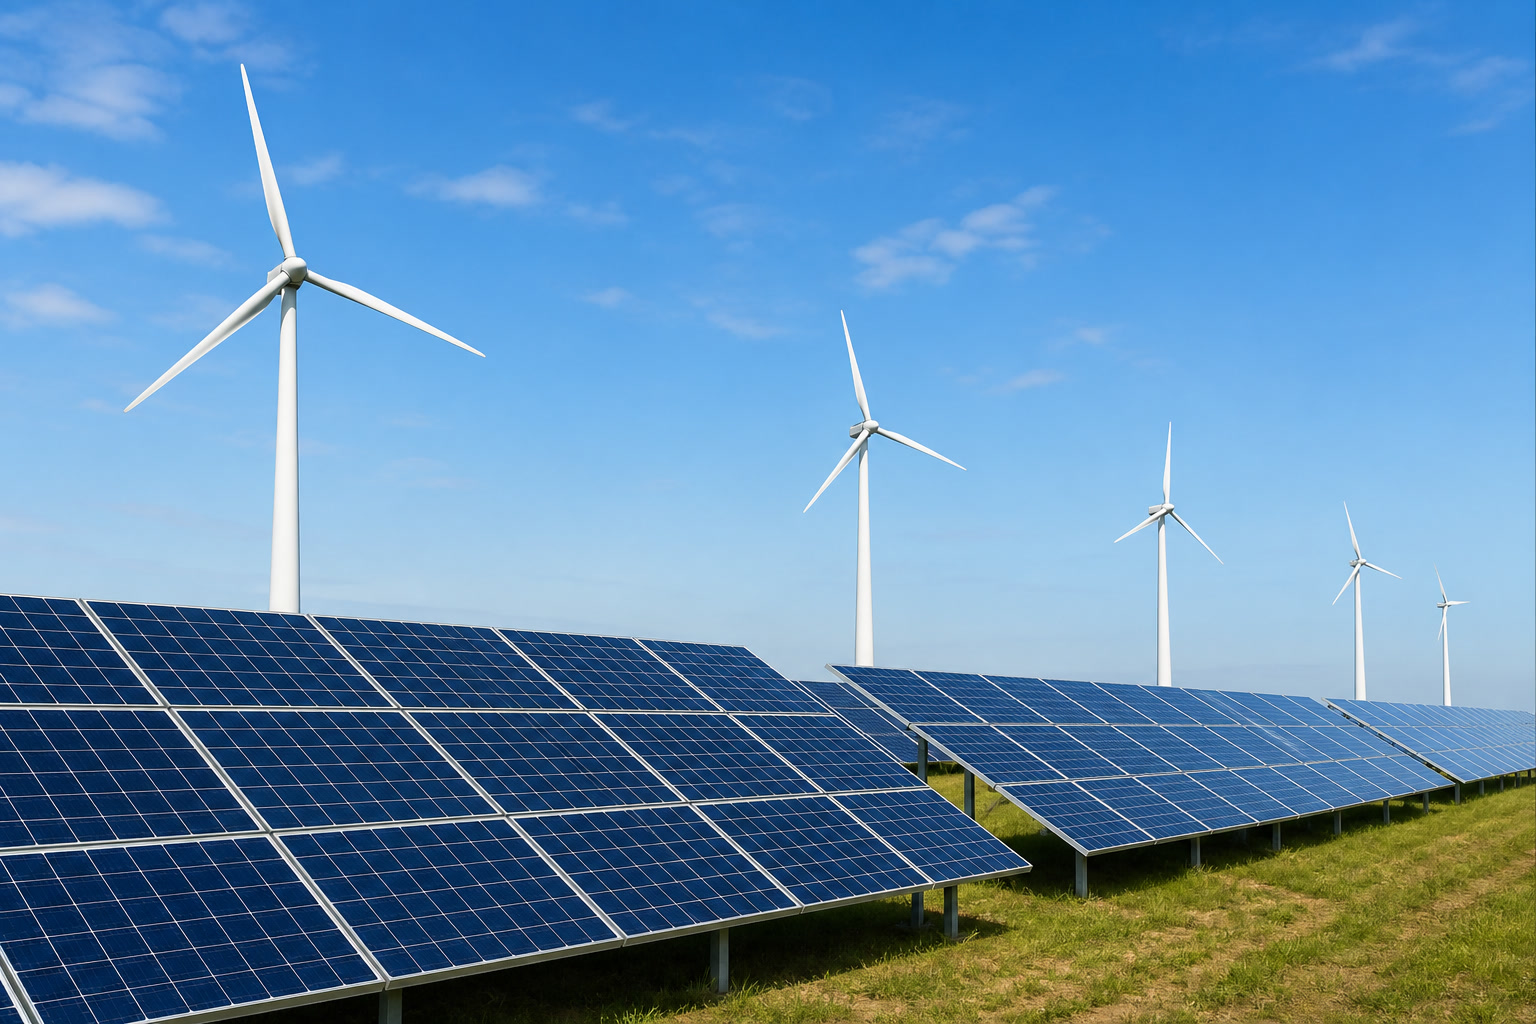
\includegraphics[width=0.55\linewidth]{images/book1/ai/g9-energy-solar-wind.jpg}

{\small 同一场地上的两台转换器：板上的阳光转化为电能，涡轮中流动的\omterm{def:g2:air-around-us:air}{空气}转化为电能。}
\end{omfigure}

\begin{remark}[“节约能量”的真正含义]\label{rem:g9:energy-conversions:saving}
若守恒定律守护着每一\omterm{def:g9:kinetic-energy-safety:joule}{焦耳}，人们为何还要“节约\omterm{def:g5:everyday-energy:energy}{能量}”？
原因在于守恒定律保持的是\emph{数量}，而非
\emph{有用性}。集中的储存——燃料、电荷、高度——
可以被消耗，化为散布于世界各处的\omterm{def:g5:heat-and-insulation:heat}{热量}；散布的\omterm{def:g5:heat-and-insulation:heat}{热量}，
尽管每一\omterm{def:g9:kinetic-energy-safety:joule}{焦耳}都依然存在，却再也无法驱动水壶或火车：
河水已经顺坡而下。文明的能源问题不在于\omterm{def:g9:kinetic-energy-safety:joule}{焦耳}短缺——
太阳给我们的\omterm{def:g5:everyday-energy:energy}{能量}是我们所需的数千倍——
问题在于如何精打细算地使用
\emph{有用的}\omterm{def:g9:kinetic-energy-safety:joule}{焦耳}。这一思想经精确表述后，
是物理学中最负盛名的故事之一，
它要等到大学阶段，
才会以其著名的名称出现。
\end{remark}

\section{练习}

\begin{exercise}[$\star$]\label{exo:g9:energy-conversions:1}
写出清单中的七种\omterm{def:g5:everyday-energy:energy}{能量}形式，
每种各举一个家庭中的例子。
\end{exercise}

\begin{exercise}[$\star$]\label{exo:g9:energy-conversions:2}
计算 $E_p$：将 \qty{2}{kg} 的水桶提升 \qty{10}{m}；
让 \qty{60}{kg} 的徒步者登上 \qty{500}{m} 高的山坡。
\end{exercise}

\begin{exercise}[$\star$]\label{exo:g9:energy-conversions:3}
阐述守恒定律，并说明它对你童年章节中的
“永动机”做了什么。
\end{exercise}

\begin{exercise}[$\star$]\label{exo:g9:energy-conversions:4}
核算单摆一次摆动中的\omterm{def:g5:everyday-energy:energy}{能量}账目：最高点处、
最低点处，以及整体上缓慢的漂移——漂移到哪里去了？
\end{exercise}

\begin{exercise}[$\star$]\label{exo:g9:energy-conversions:5}
利用 $v = \sqrt{2 g h}$，求从 \qty{5}{m} 跳板
跳下入水时的速率，并说明为何跳水者的\omterm{def:g3:measuring-mass:mass}{质量}始终不出现。
\end{exercise}

\begin{exercise}[$\star$]\label{exo:g9:energy-conversions:6}
给出\omterm{def:g9:energy-conversions:efficiency}{效率}的定义。某\omterm{ex:g6:circuits-and-safety:motor}{电动机}输入 \qty{200}{J} 的\omterm{def:g5:everyday-energy:energy}{能量}，
输出 \qty{170}{J} 的运动：求其\omterm{def:g9:energy-conversions:efficiency}{效率}，以及
其余部分的去向？
\end{exercise}

\begin{exercise}[$\star$]\label{exo:g9:energy-conversions:7}
为何老式\omterm{def:g3:first-electric-circuit:bulb}{灯泡}会被公允地称为“一台带着
爱好的暖气”？请给出两个百分数。
\end{exercise}

\begin{exercise}[$\star$]\label{exo:g9:energy-conversions:8}
写出骑车人爬坡的完整转化链——
从早餐到山顶，写明每一种\omterm{def:g5:everyday-energy:energy}{能量}形式与每一处漏失。
\end{exercise}

\begin{exercise}[$\star\star$]\label{exo:g9:energy-conversions:9}
大坝的账本：\qty{1000}{kg} 的水下落 \qty{50}{m}
穿过水轮机。求释放的 $E_p$；在
\omterm{def:g9:energy-conversions:efficiency}{效率}为百分之九十时，每吨水的电能
——以及产生
\qty{4.4e6}{W} 输出\omterm{def:g9:electric-power-energy:power}{功率}所需的每秒吨数。
\end{exercise}

\begin{exercise}[$\star\star$]\label{exo:g9:energy-conversions:10}
一个 \qty{0.5}{kg} 的球从 \qty{2}{m} 高处落下后反弹至
\qty{1.2}{m} 高。核查这次反弹：反弹前后的\omterm{def:g5:everyday-energy:energy}{能量}，
漏失的大小与去向——以及
反弹至何种高度之后，账本上将查不到\omterm{prop:g9:kinetic-energy-safety:formula}{动能}或\omterm{def:g9:energy-conversions:forms}{势能}
的任何剩余。
\end{exercise}

\begin{exercise}[$\star\star$]\label{exo:g9:energy-conversions:11}
“电梯将电能转化为\omterm{def:g9:energy-conversions:forms}{势能}，
\omterm{def:g9:energy-conversions:efficiency}{效率}为百分之九十。”求
将一个 \qty{500}{kg} 的轿厢
提升 \qty{30}{m} 所需的电能——并
用守恒定律解释多出的百分之十。
\end{exercise}

\begin{exercise}[$\star\star\star$]\label{exo:g9:energy-conversions:12}
一名半管滑板运动员从左侧坡沿静止出发，
高度为 \qty{4}{m}。预测其经过
底部时的速率，以及在右侧能达到的高度——理想
与实际两种情况下，并描绘运动及
其\omterm{def:g5:everyday-energy:energy}{能量}的长期去向。随后结合
\cref{rem:g9:energy-conversions:saving}，解释为何在坡沿处的任何推动
都无法被完全收回：世界的账本增加了什么，
而滑板运动员
又不可挽回地损失了什么？
\end{exercise}

\section{问题：游乐园的委托}

\begin{problem}[{周末问题——游乐园聘请一位
物理顾问；过山车、高塔与
不会说谎的账本}]\label{pb:g9:energy-conversions:1}
园区新增的游乐项目必须通过你的\omterm{def:g5:everyday-energy:energy}{能量}审计，
在开园之前。取 $g = \qty{9.8}{N/kg}$；忽略摩擦，
直到摩擦再也不能忽略为止。

\medskip\noindent\textbf{第一部分——大俯冲。}
一列 \qty{2000}{kg} 的过山车被绞车拉至
\qty{45}{m} 高的顶点后从静止释放。
\begin{enumerate}
  \item 列车在顶点时的 $E_p$ 是多少？
  \item 用\omterm{def:g3:measuring-mass:mass}{质量}可约去的公式，求俯冲底部的理想速率，
        以 \unit{m/s} 与
        \unit{km/h} 表示？
  \item 设计者又增设了一座 \qty{50}{m} 高的
        第二座小山，紧接在俯冲之后。请用账本否决它——
        并写出理想列车所能
        翻越的最高第二座小山的高度。
  \item 实测的底部速率为 \qty{28}{m/s}，而非
        理想值。求出两种情况下的\omterm{prop:g9:kinetic-energy-safety:formula}{动能}，并
        将差值记入相应账目。
\end{enumerate}

\medskip\noindent\textbf{第二部分——绞车与
账单。}
\begin{enumerate}[resume]
  \item 绞车将列车拉升至顶点，耗时
        \qty{60}{s}。若\omterm{def:g9:energy-conversions:efficiency}{效率}为百分之百，其\omterm{def:g9:electric-power-energy:power}{功率}是多少？
  \item 实际绞车的\omterm{def:g9:electric-power-energy:power}{功率}为 \qty{20}{kW}。其
        \omterm{def:g9:energy-conversions:efficiency}{效率}是多少？
  \item 每趟每四分钟运行一次，每天运行
        十\omterm{ex:g2:measuring-time:clock}{小时}。绞车的每日耗能（以\omterm{def:g9:electric-power-energy:kwh}{千瓦时}计，
        实际绞车，计入提升次数），以及其
        每\omterm{def:g6:measurement-in-science:measuring}{单位} $0.25$ 时的费用是多少？
  \item 有设计者提议回收列车
        到站时的\omterm{def:g5:everyday-energy:energy}{能量}，用发电制动器馈入电网——
        “游乐项目能够自负盈亏！”请核算这一设想：
        现实中能回收多大比例，以及
        哪条定律禁止完整的循环？
\end{enumerate}

\medskip\noindent\textbf{第三部分——自由落体塔
与报告。}
\qty{60}{m} 高的塔使一个 \qty{500}{kg} 的吊舱
下落，并在 \qty{10}{m} 处进入磁力制动器。
\begin{enumerate}[resume]
  \item 进入制动区时的速率（理想自由下落
        \qty{50}{m}）？
  \item 制动器必须耗散的\omterm{def:g5:everyday-energy:energy}{能量}，以及感应
        将其导向何处。（制动器是\omterm{def:g9:alternator:alternator}{交流发电机}一章的
        近亲——感应电流产生的涡流
        使金属发热。）
  \item 乘客尖叫着说，下落过程中他们感到“失重”，
        请依据\omterm{def:g9:gravitation:gravitation}{万有引力}一章中“落体同伴”的想法，
        以一句
        话裁定这一说法。
  \item 请在委托报告上签字：三句话——
        过山车赖以运行的那笔“交易”，每个游乐项目
        所遵守的定律，以及悄悄向它们全部征税的
        那笔账。
\end{enumerate}
\end{problem}
